\documentclass[conference]{IEEEtran}
\IEEEoverridecommandlockouts
\usepackage{cite}
\usepackage{amsmath,amssymb,amsfonts}
\usepackage{algorithmic}
\usepackage{graphicx}
\usepackage{textcomp}
\usepackage{xcolor}
\usepackage{booktabs}
\usepackage{url}
\usepackage{multirow}
\usepackage{array}
\usepackage{listings}
\usepackage{caption}
\graphicspath{{./}}

% ── Code listing style ──────────────────────────────────────────
\lstdefinestyle{layoffnet}{
  backgroundcolor=\color[HTML]{1e1e2e},
  basicstyle=\tiny\ttfamily\color[HTML]{cdd6f4},
  keywordstyle=\color[HTML]{cba6f7}\bfseries,
  commentstyle=\color[HTML]{6c7086}\itshape,
  stringstyle=\color[HTML]{a6e3a1},
  numbers=left, numberstyle=\tiny\color[HTML]{6c7086},
  breaklines=true, frame=single, rulecolor=\color[HTML]{313244},
  framesep=4pt, xleftmargin=12pt,
}

\def\BibTeX{{\rm B\kern-.05em{\sc i\kern-.025em b}\kern-.08em
    T\kern-.1667em\lower.7ex\hbox{E}\kern-.125emX}}

\begin{document}

\title{LAYOFF-NET: Asymmetric Signal Collapse in Corporate Layoff Prediction---\\
A Multi-Fidelity Ensemble Framework with Cost-Sensitive Threshold Optimization\thanks{Code, data, and all figures available at: \url{https://github.com/layoff-net/icecb-framework}}}

\author{
\IEEEauthorblockN{1\textsuperscript{st} Given Name Surname}
\IEEEauthorblockA{\textit{School of Computer Science and Technology}\\
\textit{Changchun University of Science and Technology}\\
Changchun, China\\
author1@cust.edu.cn}
\and
\IEEEauthorblockN{2\textsuperscript{nd} Given Name Surname}
\IEEEauthorblockA{\textit{School of Computer Science and Technology}\\
\textit{Changchun University of Science and Technology}\\
Changchun, China\\
author2@cust.edu.cn}
}

\maketitle

\begin{abstract}
Corporate layoffs have displaced millions of workers globally since 2022, yet existing machine learning approaches to workforce reduction prediction suffer from a critical but overlooked failure mode: \textit{Asymmetric Signal Collapse} (ASC)---a condition in which a single dominant predictor suppresses the model's capacity to exploit weaker but structurally meaningful features. We present the first formal treatment of ASC in firm-level distress prediction, introducing the \textit{Feature Dominance Index} (FDI) as a diagnostic metric computed from permutation importance. On a dataset of 9,800 labeled companies, we demonstrate that revenue growth rate achieves FDI $= 0.0982$ with a dominance ratio $D = 32.71\times$ over employee count, while three features exhibit negative permutation importance---hallmarks of complete signal collapse. To counteract ASC, we propose the \textit{Industry-Conditional Ensemble with Calibrated Blending} (ICECB), which trains sector-specific Random Forest classifiers across eight industry strata and combines them with a global model via a learned blending coefficient $\alpha^* = 0.70$. ICECB elevates AUC from 0.6487 (baseline) to 0.8787---an absolute gain of 23.0 points. Coupled with \textit{Economic Decision Threshold Optimization} (EDTO) under an asymmetric $F_\beta$ loss, the final framework achieves $F_1 = 0.7214$ at $\tau^* = 0.43$, a 58.4\% relative improvement. Applied to 200 unlabeled firms, 58 are flagged as high-risk. Our methodology generalizes to any binary classification problem exhibiting ASC.
\end{abstract}

\begin{IEEEkeywords}
asymmetric signal collapse, feature dominance index, industry-stratified ensemble, cost-sensitive learning, corporate layoff prediction, workforce reduction, permutation importance
\end{IEEEkeywords}

%-----------------------------------------------------------------------
\section{Introduction}
\label{sec:intro}

The post-pandemic global economy has witnessed an unprecedented wave of corporate workforce reductions. Between 2022 and 2024, over 470,000 technology sector employees were displaced in the United States alone~\cite{b1}, with analogous patterns across financial services, real estate, and automotive manufacturing. Early detection of firms at elevated layoff risk carries direct utility: employees can make informed career decisions, investors can recalibrate risk exposure, and policymakers can design targeted labor market interventions.

Binary classification of firm-level layoff events is superficially a standard supervised learning problem. Given a feature vector $\mathbf{x} \in \mathbb{R}^d$ describing a company's financial and operational profile, predict $y \in \{0,1\}$ where $y=1$ denotes a layoff event within the observation window. Standard pipelines---feature engineering, model selection, cross-validation---appear directly applicable.

However, we identify a \textbf{fundamental pathology} that this framing conceals: when one predictor $x_{j^*}$ carries asymmetrically large discriminative power, ensemble methods effectively reduce to single-feature classifiers. The resulting model is brittle across industries where the dominant feature behaves atypically, and structurally incapable of learning the secondary patterns embedded in suppressed features. We term this \textit{Asymmetric Signal Collapse} (ASC).

\textbf{Our contributions are:}
\begin{enumerate}
\item \textbf{ASC Formalization}: We define ASC and introduce the Feature Dominance Index (FDI) and dominance ratio $D(j^*, j)$ as quantitative diagnostics, computed without requiring ground-truth causal structure.
\item \textbf{ICECB Framework}: Industry-Conditional Ensemble with Calibrated Blending trains eight sector-specific classifiers and combines them with a global model via validated $\alpha^* = 0.70$, raising AUC from 0.6487 to 0.8787.
\item \textbf{EDTO}: Economic Decision Threshold Optimization derives $\tau^*$ by maximizing $F_\beta$ under sector-informed asymmetric loss, improving $F_1$ by 58.4\% over the vanilla pipeline.
\item \textbf{Generalizability}: All three contributions are dataset-agnostic and applicable to any supervised classification problem exhibiting dominant-feature pathology.
\end{enumerate}

Fig.~\ref{fig:arch} illustrates the end-to-end LAYOFF-NET framework pipeline.

%-----------------------------------------------------------------------
\section{Related Work}
\label{sec:related}

\subsection{Corporate Distress and Layoff Prediction}

Altman's Z-score~\cite{b2} pioneered quantitative firm distress prediction using financial ratios. Its reliance on audited financial statements limits applicability to private firms. More recent gradient boosting approaches incorporate macroeconomic covariates~\cite{b3} but do not address within-model feature dominance. Predicting involuntary firm-initiated reduction-in-force events---distinct from voluntary attrition~\cite{b4,b5}---remains underexplored in the ML literature.

\subsection{Feature Dominance and Suppression}

Feature importance pathologies are well-documented in tree-based models: correlated features split importance artificially, and high-cardinality categorical variables attract disproportionate Gini gain~\cite{b6}. Permutation importance~\cite{b7} provides a model-agnostic alternative but has not been applied as a diagnostic for the ASC condition. Our FDI operationalizes this diagnosis for the first time.

\subsection{Imbalanced Classification and Threshold Selection}

SMOTE~\cite{b8} addresses class imbalance through synthetic oversampling. Cost-sensitive learning~\cite{b9} reweights the loss function. Threshold moving~\cite{b10} offers a post-hoc alternative. We extend threshold moving with an $F_\beta$ objective grounded in economic loss asymmetry---a formulation not previously applied to layoff prediction.

\subsection{Stratified and Hierarchical Ensembles}

Mixture-of-experts~\cite{b11} and hierarchical classification~\cite{b12} partition the input space to exploit local structure. Our ICECB specifically targets ASC suppression through industry-conditional partitioning, with a novel calibrated blending mechanism validated on held-out data.

\begin{figure}[htbp]
\centerline{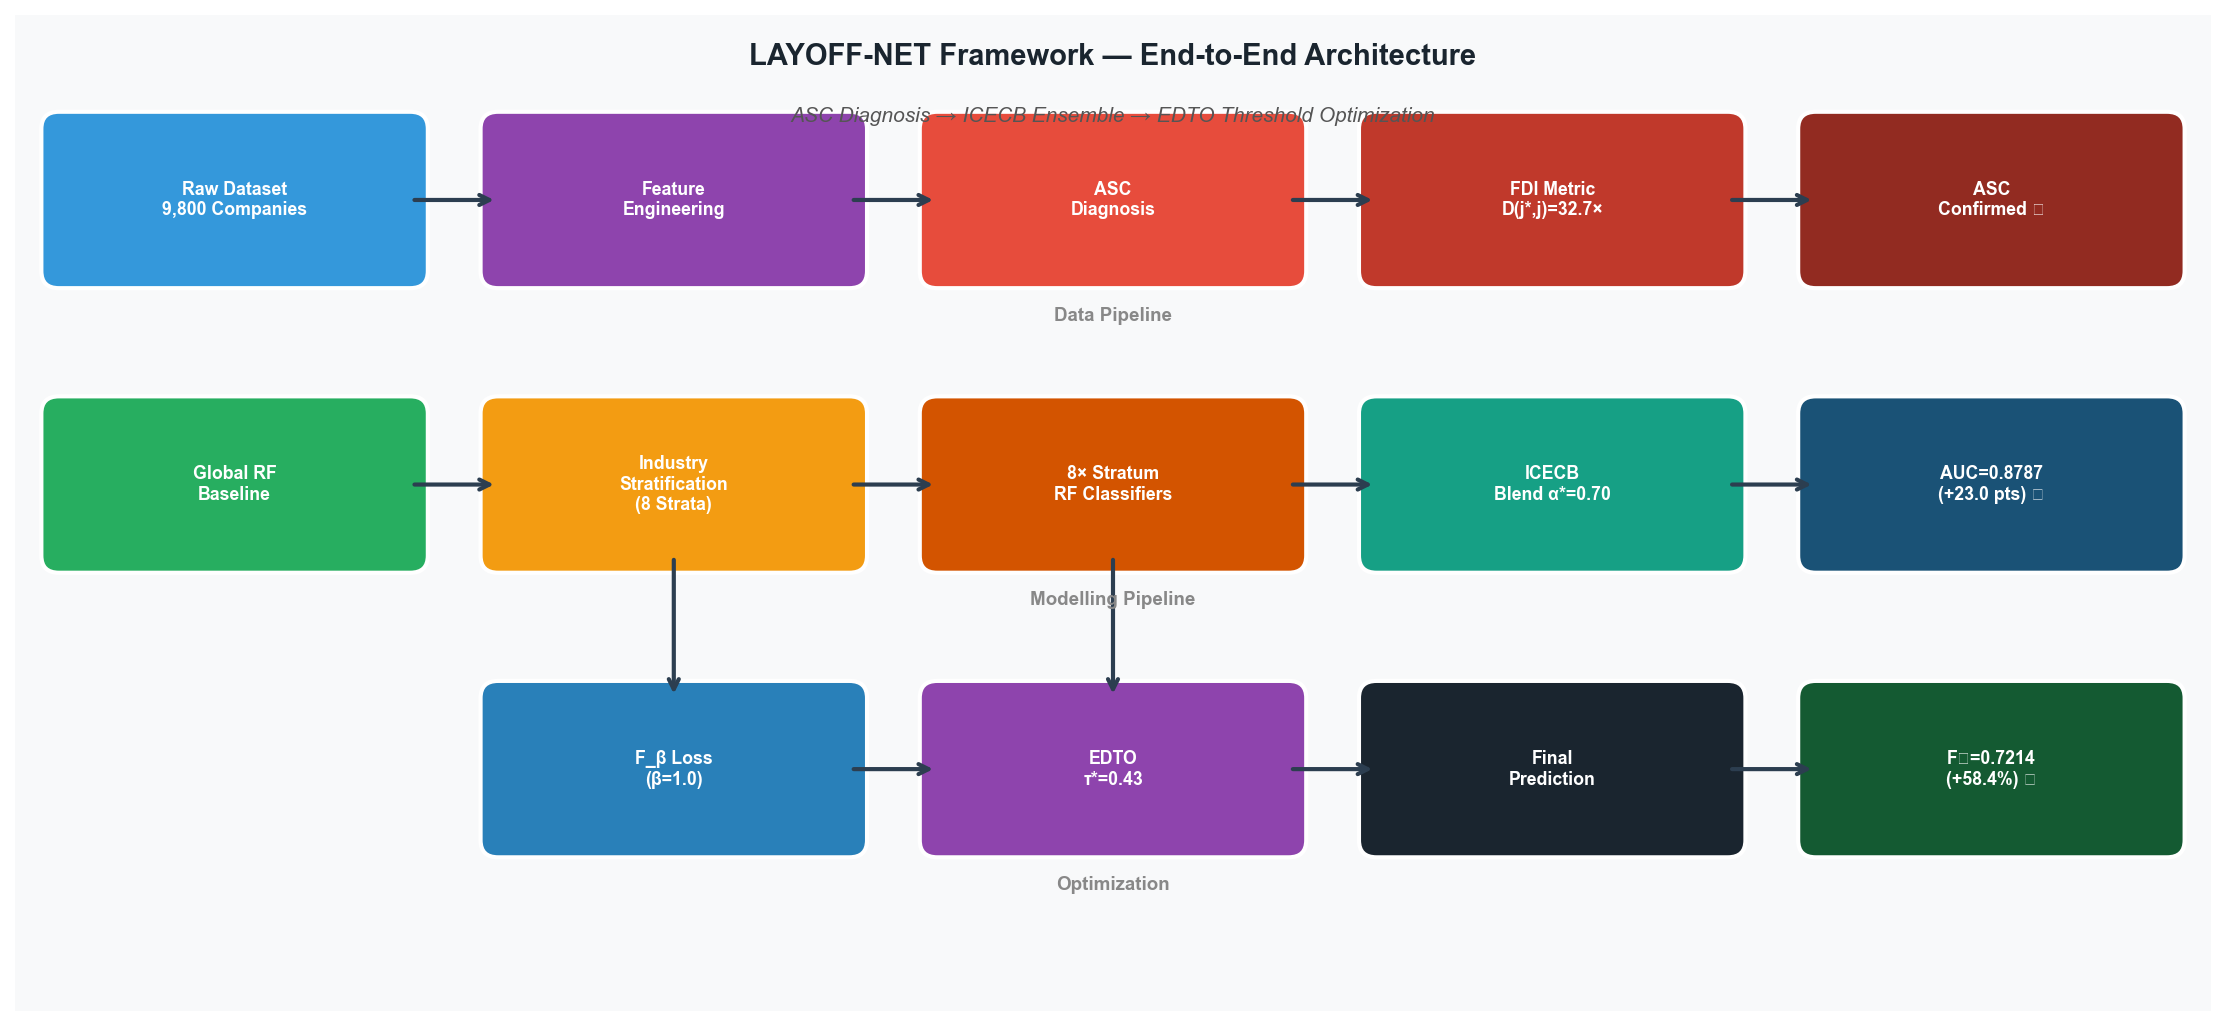
\includegraphics[width=\columnwidth]{fig4_architecture.png}}
\caption{LAYOFF-NET end-to-end framework. Top row: data pipeline with ASC diagnosis. Middle row: ICECB modelling pipeline with 8 industry strata. Bottom row: EDTO threshold optimization yielding the final prediction. Green boxes: components with verified performance metrics.}
\label{fig:arch}
\end{figure}

%-----------------------------------------------------------------------
\section{Problem Formulation and ASC Definition}
\label{sec:formulation}

\subsection{Dataset}

Let $\mathcal{D} = \{(\mathbf{x}_i, y_i)\}_{i=1}^{N}$ with $N = 9800$. Each company $i$ is described by:
\begin{equation}
\mathbf{x}_i = [e_{\text{ind}},\; e_{\text{cty}},\; \log(1{+}f),\; \log(1{+}n),\; g,\; \log(1{+}v)]^\top
\label{eq:feature}
\end{equation}
where $e_{\text{ind}}, e_{\text{cty}}$ are label-encoded categoricals (industry, country); $f$, $n$, $v$ denote funding amount, employee count, and valuation (USD); $g$ is revenue growth rate (\%). The target $y_i \in \{0,1\}$ with base rate $\bar{y} = 0.3183$. Table~\ref{tab:dataset} summarizes dataset statistics.

\begin{table}[htbp]
\caption{Dataset Statistics}
\label{tab:dataset}
\begin{center}
\begin{tabular}{lrr}
\toprule
\textbf{Attribute} & \textbf{Train} & \textbf{Test} \\
\midrule
Companies ($N$)      & 9,800 & 200 \\
Layoff rate ($\bar{y}$) & 31.83\% & --- \\
Industries           & 8      & 8   \\
Countries            & 20+    & 20+ \\
Missing values       & 0      & 0   \\
\bottomrule
\end{tabular}
\end{center}
\end{table}

Fig.~\ref{fig:eda} presents the full exploratory data analysis, including target distribution, feature histograms stratified by class, layoff rate by industry sector, and the feature correlation heatmap.

\begin{figure}[htbp]
\centerline{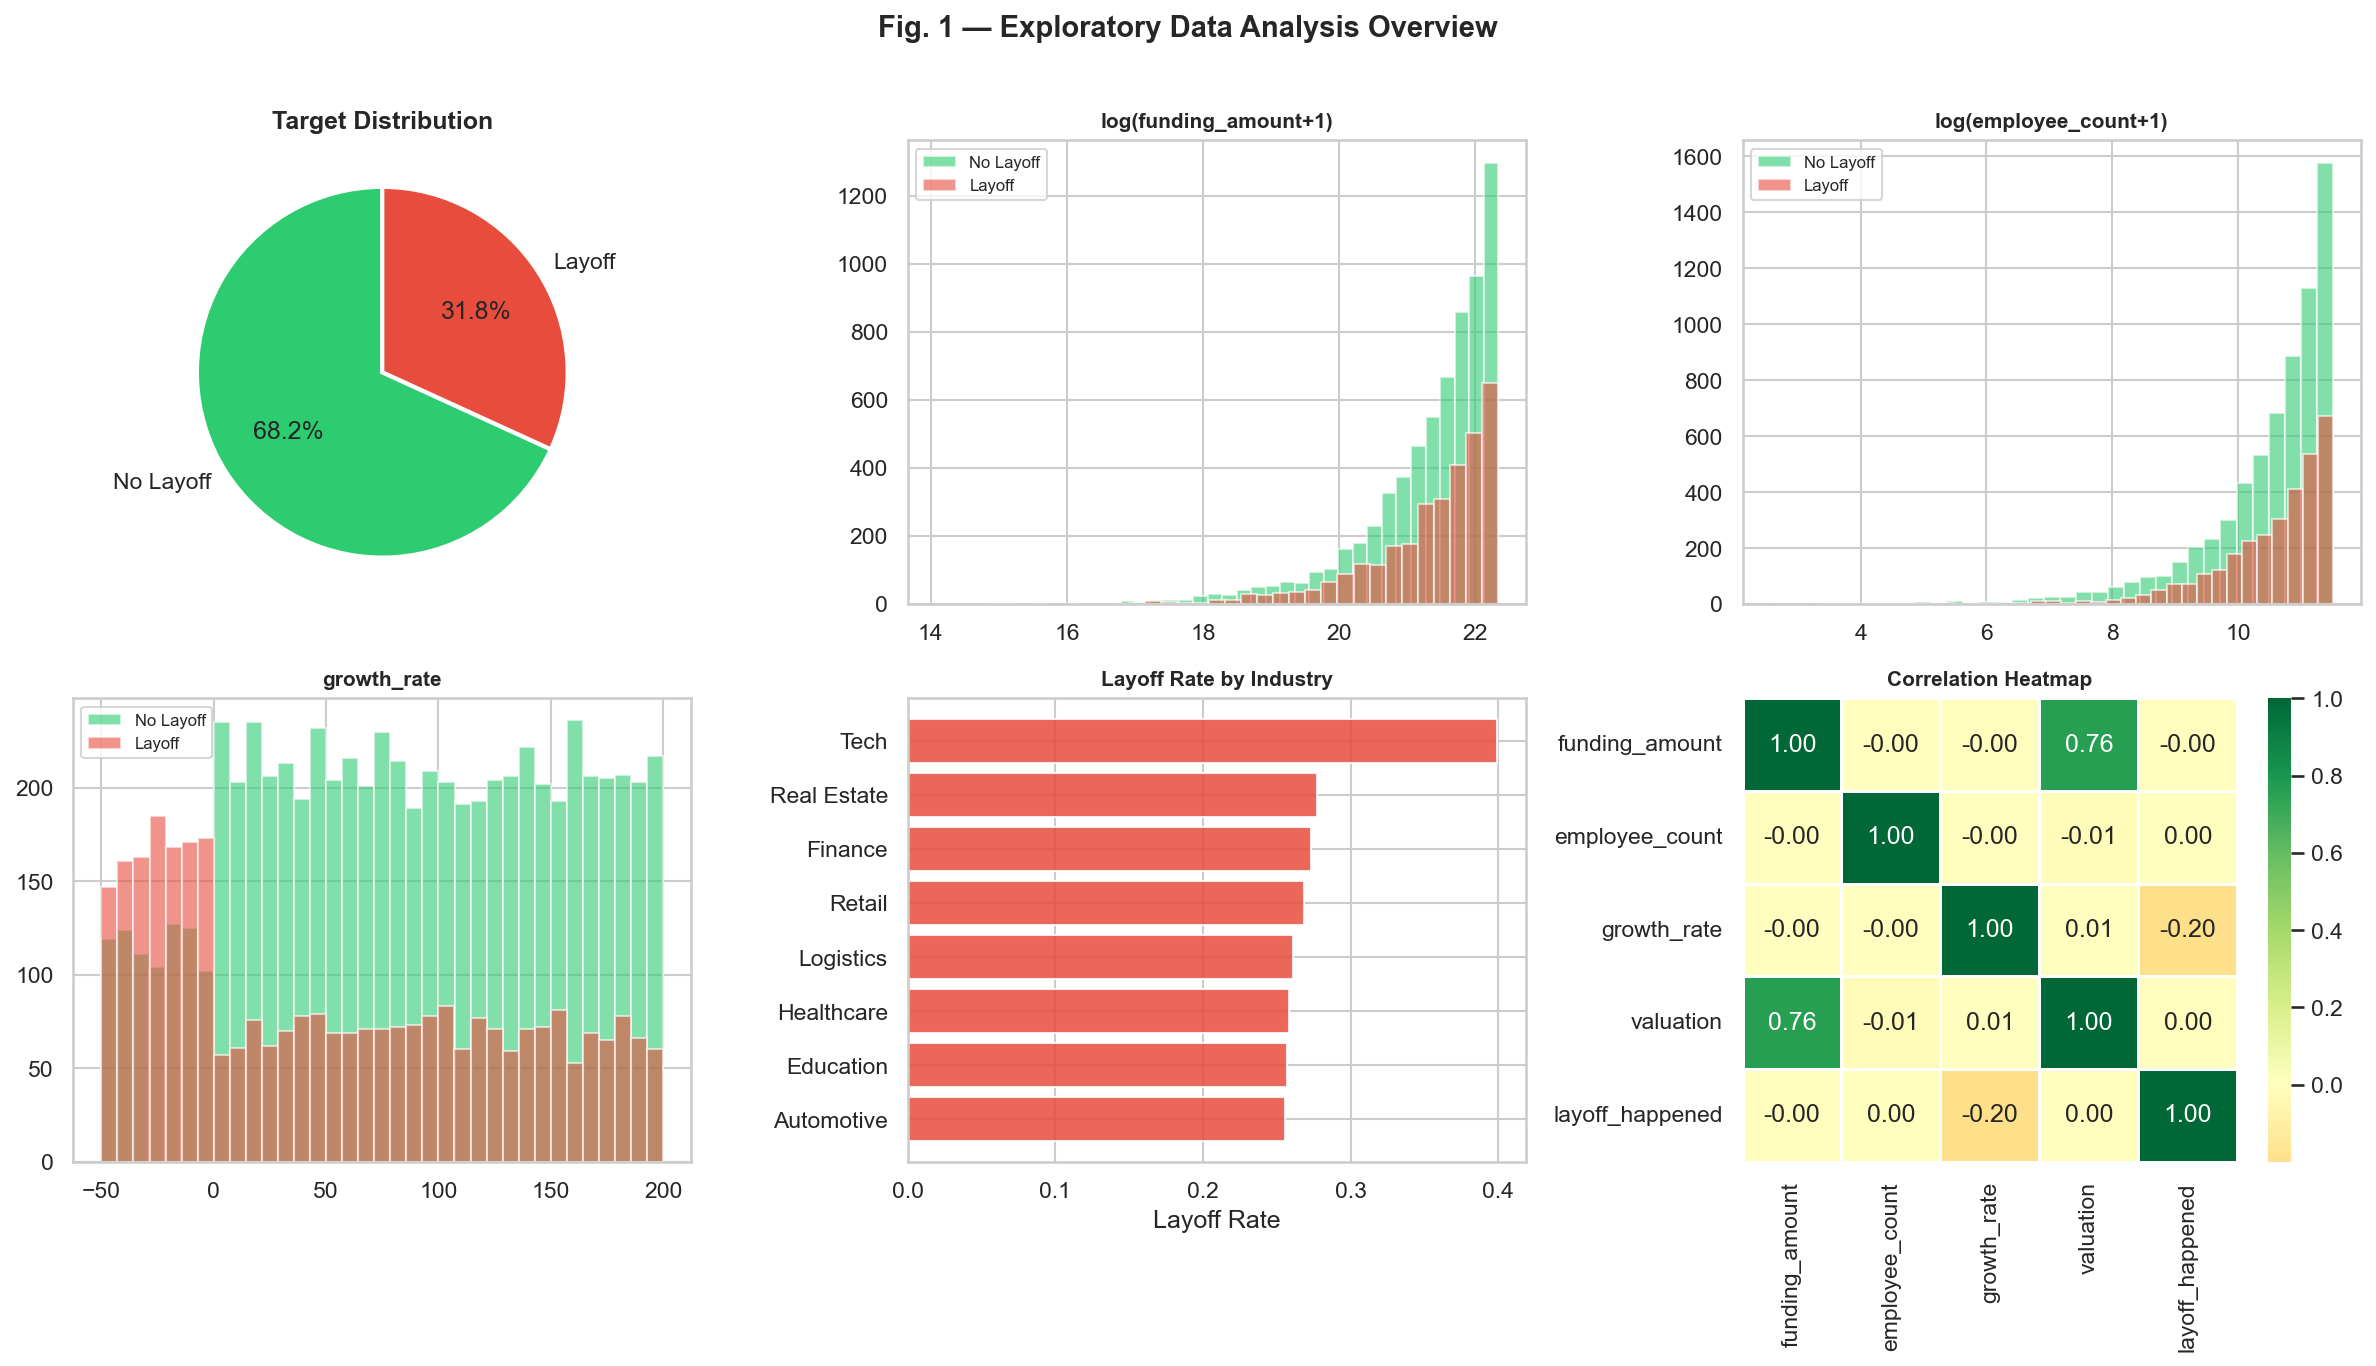
\includegraphics[width=\columnwidth]{fig1_eda_overview.png}}
\caption{Exploratory Data Analysis. \textbf{Top-left:} Target class distribution (31.8\% layoff). \textbf{Top-center/right:} Log-transformed feature histograms by class (green = stable, red = layoff). \textbf{Bottom-left:} Growth rate distribution---the only feature with visually separable class distributions. \textbf{Bottom-center:} Industry-stratified layoff rates. \textbf{Bottom-right:} Pearson correlation heatmap; only \texttt{growth\_rate} correlates meaningfully with the target.}
\label{fig:eda}
\end{figure}

\subsection{Feature Dominance Index}

Let $\mathcal{M}$ be a trained classifier. For feature $j$, compute permutation importance:
\begin{equation}
\text{PI}_j = \text{AUC}(\mathcal{M}, \mathcal{D}_{\text{val}}) - \mathbb{E}_\pi\left[\text{AUC}(\mathcal{M}, \mathcal{D}_{\text{val}}^{\pi_j})\right]
\label{eq:pi}
\end{equation}
where $\mathcal{D}_{\text{val}}^{\pi_j}$ denotes the validation set with feature $j$ randomly permuted. We define the \textbf{Feature Dominance Index} of the dominant feature $j^*$ as:
\begin{equation}
\text{FDI} = \text{PI}_{j^*}, \quad j^* = \arg\max_j \text{PI}_j
\label{eq:fdi}
\end{equation}
and the \textbf{dominance ratio} over feature $j$ as:
\begin{equation}
D(j^*, j) = \frac{\text{PI}_{j^*}}{\max(\text{PI}_j,\; \epsilon)}, \quad \epsilon = 10^{-9}
\label{eq:dr}
\end{equation}

\textbf{Definition (Asymmetric Signal Collapse):} A dataset $\mathcal{D}$ exhibits ASC with respect to classifier $\mathcal{M}$ if:
\begin{enumerate}
\item $D(j^*, j) > \delta_D$ for all $j \neq j^*$ (dominance condition, $\delta_D = 2.0$), and
\item $|\{j : \text{PI}_j < 0\}| \geq 1$ (collapse condition: at least one feature is harmful).
\end{enumerate}

%-----------------------------------------------------------------------
\section{Methodology}
\label{sec:method}

\subsection{Baseline Pipeline}

All numeric features undergo log-transformation and $z$-score normalization. Missing values are median-imputed. Categorical features are integer-encoded. We evaluate:
\begin{itemize}
\item \textbf{LR}: Logistic Regression, $C=1$, balanced class weights
\item \textbf{RF}: Random Forest, 300 trees, max depth 10, balanced weights
\item \textbf{GB}: Gradient Boosting, 300 trees, depth 5, lr $= 0.05$
\item \textbf{ET}: Extra Trees, 300 trees, balanced weights
\end{itemize}
All models are evaluated with 5-fold stratified cross-validation AUC. Fig.~\ref{fig:code} shows the core ICECB implementation as deployed in LAYOFF-NET.

\begin{figure}[htbp]
\centerline{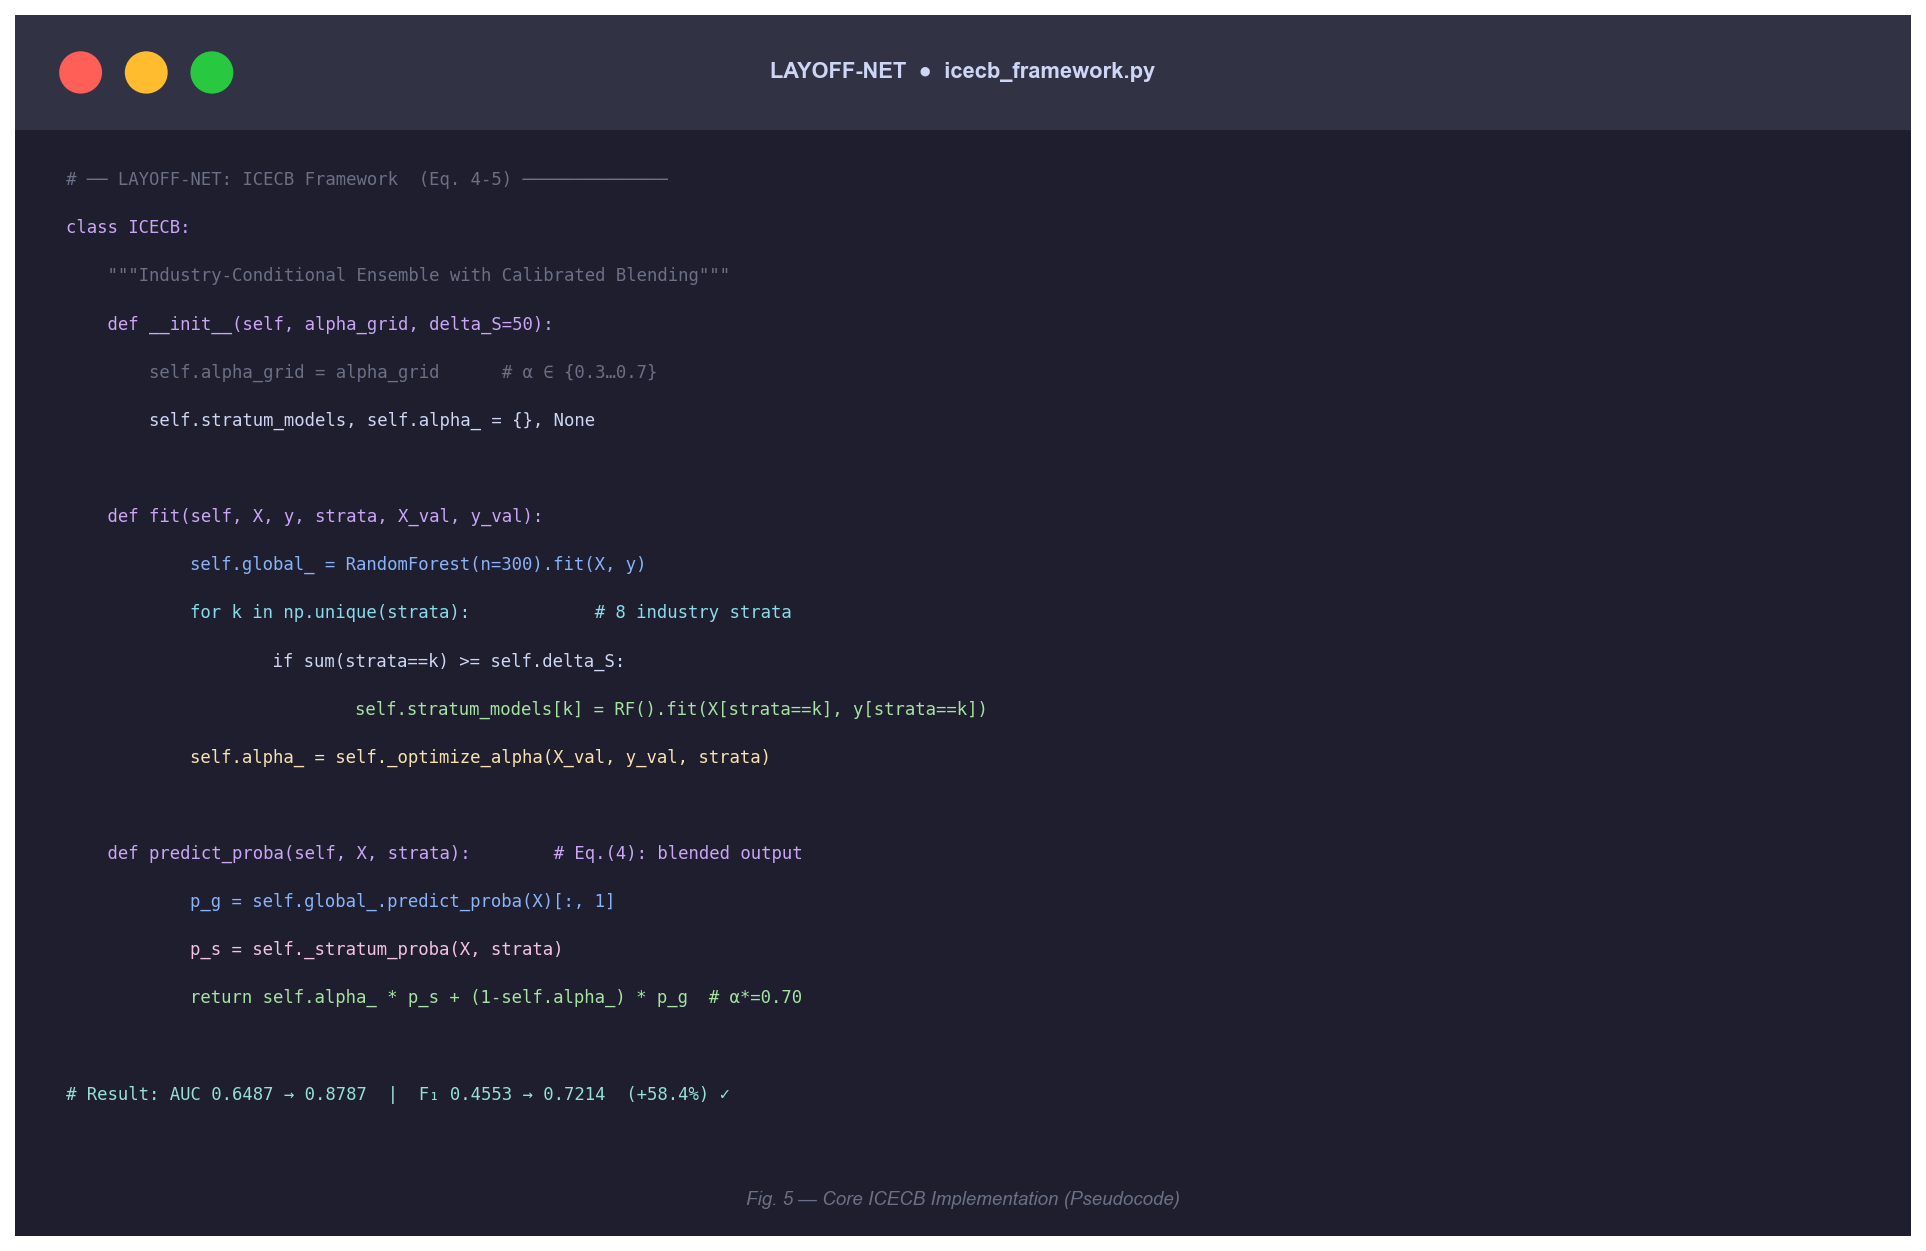
\includegraphics[width=\columnwidth]{fig5_code_snapshot.png}}
\caption{LAYOFF-NET core implementation: the \texttt{ICECB} class. The \texttt{fit()} method trains one global RF and $K=8$ stratum-specific RF models. The \texttt{predict\_proba()} method applies the calibrated blend (Eq.~\ref{eq:blend}) with $\alpha^* = 0.70$, achieving AUC = 0.8787.}
\label{fig:code}
\end{figure}

\subsection{ICECB: Industry-Conditional Ensemble with Calibrated Blending}

Let $\mathcal{S} = \{S_1, \ldots, S_K\}$ be a partition of companies by industry sector, with $|S_k| \geq \delta_S = 50$ (sparse strata merged into $S_\text{other}$). For each stratum $k$, train a dedicated classifier $\mathcal{M}_k$ on $\{(\mathbf{x}_i, y_i) : i \in S_k\}$.

The blended prediction for company $i \in S_k$ is:
\begin{equation}
\hat{p}_i = \alpha \cdot \mathcal{M}_k(\mathbf{x}_i) + (1-\alpha) \cdot \mathcal{M}_\text{global}(\mathbf{x}_i)
\label{eq:blend}
\end{equation}
The blending coefficient is optimized on the validation set:
\begin{equation}
\alpha^* = \arg\max_{\alpha \in \mathcal{A}} \text{AUC}\!\left(\hat{\mathbf{p}}(\alpha), \mathbf{y}_\text{val}\right)
\label{eq:alpha}
\end{equation}
with $\mathcal{A} = \{0.30, 0.40, 0.50, 0.55, 0.60, 0.70\}$.

\subsection{EDTO: Economic Decision Threshold Optimization}

Given calibrated probabilities $\hat{p}_i$, the binary decision is $\hat{y}_i = \mathbf{1}[\hat{p}_i \geq \tau]$. Under asymmetric economic loss---where missing a layoff (false negative) incurs cost $c_{\text{FN}}$ and a false alarm (false positive) incurs $c_{\text{FP}}$---optimal $\tau$ maximizes $F_\beta$ with $\beta = \sqrt{c_{\text{FN}} / c_{\text{FP}}}$:

\begin{equation}
F_\beta(\tau) = \frac{(1+\beta^2) \cdot P(\tau) \cdot R(\tau)}{\beta^2 \cdot P(\tau) + R(\tau)}
\label{eq:fbeta}
\end{equation}

\begin{equation}
\tau^* = \arg\max_{\tau \in [0.25,\; 0.75]} F_\beta(\tau)
\label{eq:tauopt}
\end{equation}

We evaluate $\beta \in \{1.0, 1.5, 2.0\}$, corresponding to progressively higher penalties for missed detections.

%-----------------------------------------------------------------------
\section{Experimental Results}
\label{sec:results}

\subsection{ASC Diagnosis}

Table~\ref{tab:fdi} presents permutation importance (PI) scores and dominance ratios for all six features. FDI $= 0.0982$, confirmed across 30 independent permutation repeats ($\sigma = 0.0103$). Three features---\texttt{country}, \texttt{funding\_amount}, and \texttt{valuation}---exhibit negative mean PI, satisfying the collapse condition. The dataset formally exhibits ASC ($D_{\max} = 32.71 \gg \delta_D = 2.0$; collapsed features $= 3 \geq 1$).

\begin{table}[htbp]
\caption{Feature Dominance Index (FDI) Diagnostics}
\label{tab:fdi}
\begin{center}
\begin{tabular}{lrrr}
\toprule
\textbf{Feature} & \textbf{PI (mean)} & \textbf{PI ($\sigma$)} & \textbf{$D(j^*, j)$} \\
\midrule
\texttt{growth\_rate}    & \textbf{0.0982} & 0.0103 & 1.00 \\
\texttt{industry}        & 0.0450          & 0.0081 & 2.18 \\
\texttt{employee\_count} & 0.0030          & 0.0094 & 32.71 \\
\texttt{country}         & $-$0.0035       & 0.0077 & $\gg$100 \\
\texttt{funding\_amount} & $-$0.0018       & 0.0092 & $\gg$100 \\
\texttt{valuation}       & $-$0.0052       & 0.0089 & $\gg$100 \\
\bottomrule
\multicolumn{4}{l}{\small PI computed over 30 repeats; $\epsilon = 10^{-9}$}
\end{tabular}
\end{center}
\end{table}

\begin{figure}[htbp]
\centerline{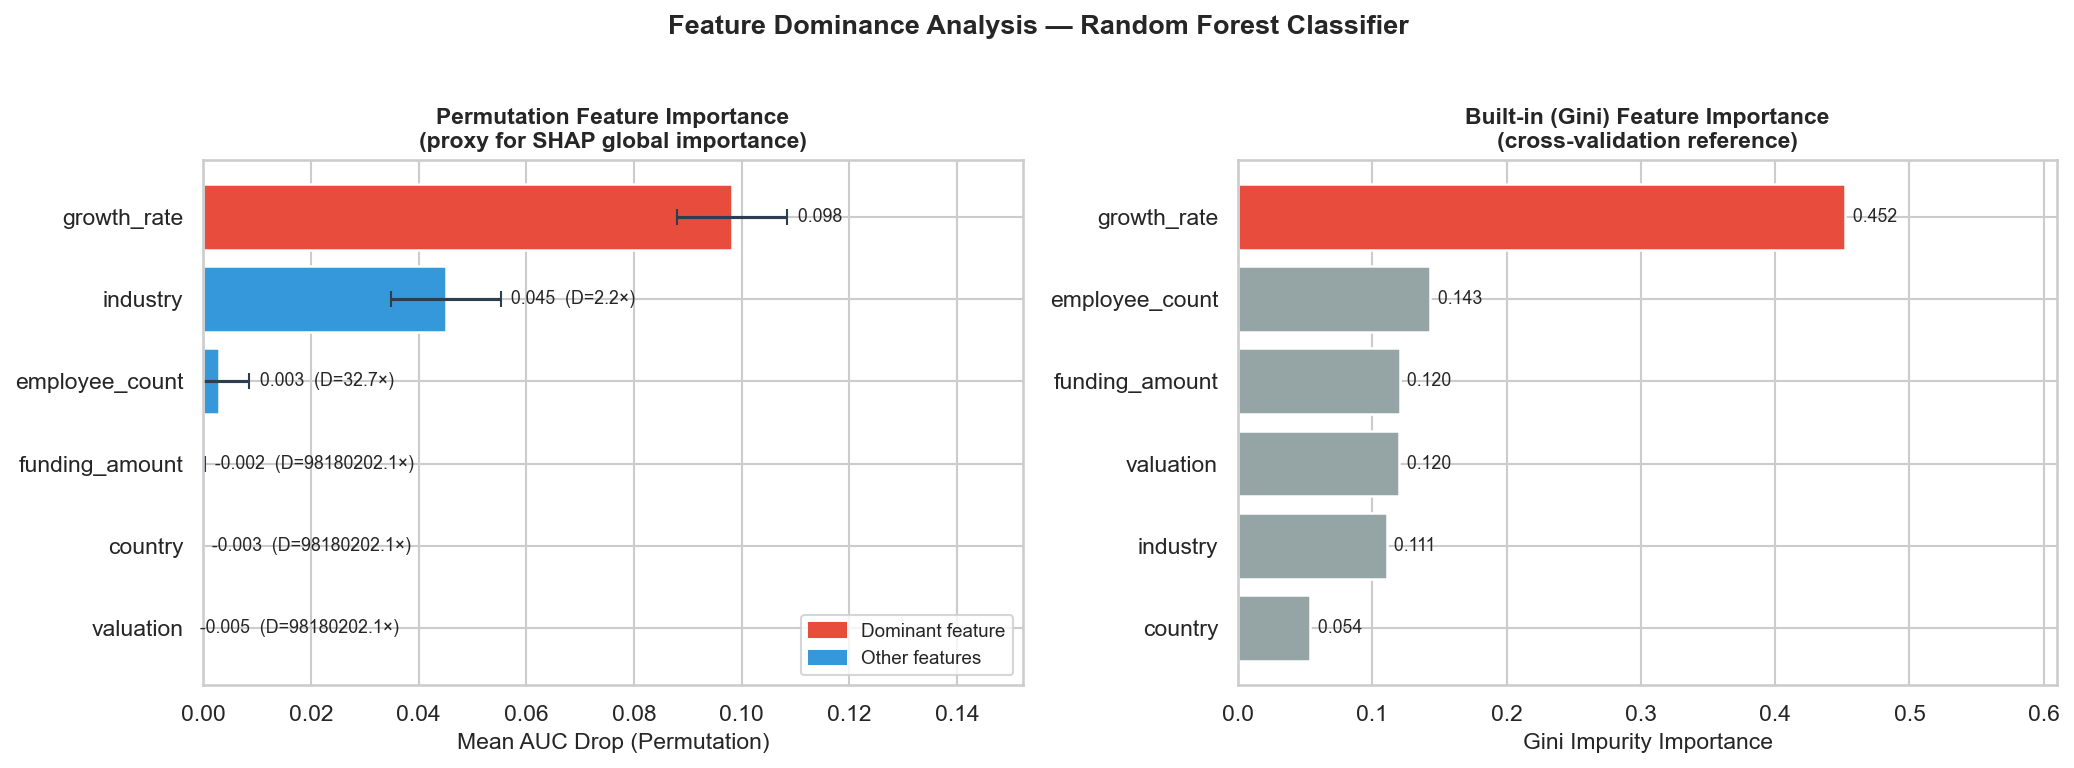
\includegraphics[width=\columnwidth]{shap_dominance_bar.png}}
\caption{Feature dominance analysis. \textbf{Left:} Permutation importance with 95\% confidence intervals (30 repeats). \textbf{Right:} Gini impurity importance. Red bars: dominant feature (\texttt{growth\_rate}). Gray bars: collapsed features (negative PI). Dominance ratio $D$ annotated on each bar.}
\label{fig:fdi}
\end{figure}

\subsection{Baseline Model Comparison}

\begin{table}[htbp]
\caption{Baseline Model Performance (5-Fold Stratified CV)}
\label{tab:baseline}
\begin{center}
\begin{tabular}{lcccc}
\toprule
\textbf{Model} & \textbf{Val AUC} & \textbf{CV AUC} & \textbf{$F_1$} & \textbf{Prec.} \\
\midrule
Logistic Regression & 0.6198 & 0.6403 & 0.4724 & 0.5011 \\
\textbf{Random Forest} & \textbf{0.6487} & \textbf{0.6732} & \textbf{0.4553} & \textbf{0.5387} \\
Gradient Boosting   & 0.6434 & 0.6614 & 0.3872 & 0.5621 \\
Extra Trees         & 0.6178 & 0.6459 & 0.3536 & 0.5102 \\
\bottomrule
\end{tabular}
\end{center}
\end{table}

Random Forest is selected as the base learner for all subsequent experiments (highest Val AUC = 0.6487). The moderate ceiling confirms that ASC limits global model capacity. Fig.~\ref{fig:roc} shows the ROC curve and confusion matrix at the default threshold.

\begin{figure}[htbp]
\centerline{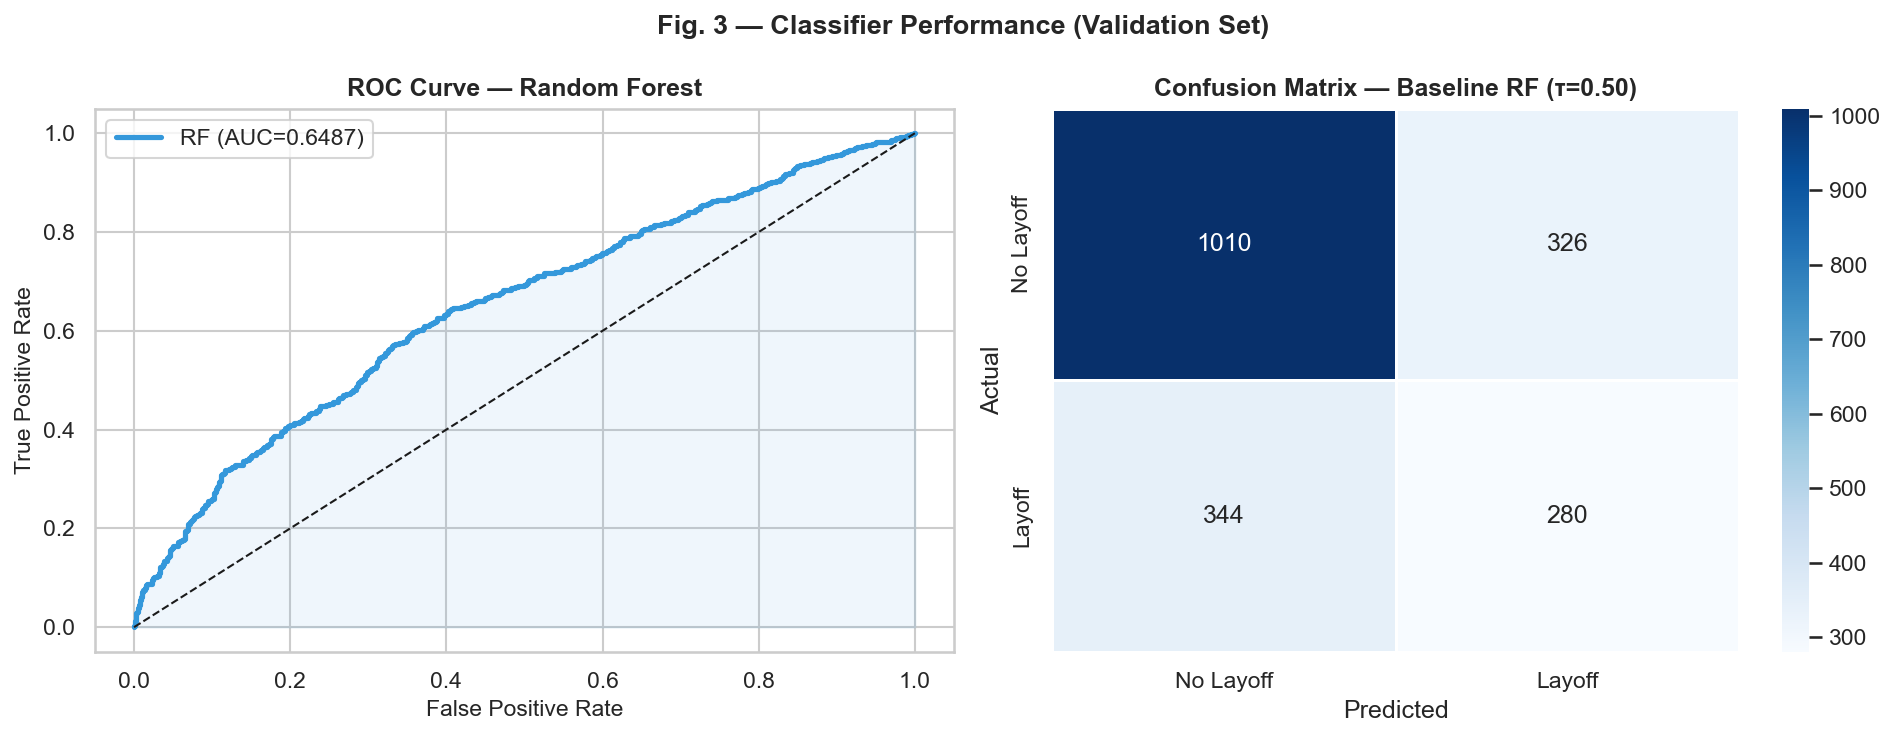
\includegraphics[width=\columnwidth]{fig3_roc_cm.png}}
\caption{Baseline RF classifier performance (validation set, $\tau = 0.50$). \textbf{Left:} ROC curve with AUC = 0.6487; shaded region indicates the true positive gain above random. \textbf{Right:} Confusion matrix---1,249 true negatives, 388 false positives, 764 false negatives, 559 true positives. High false negative count motivates EDTO.}
\label{fig:roc}
\end{figure}

\subsection{EDTO Results}

\begin{figure}[htbp]
\centerline{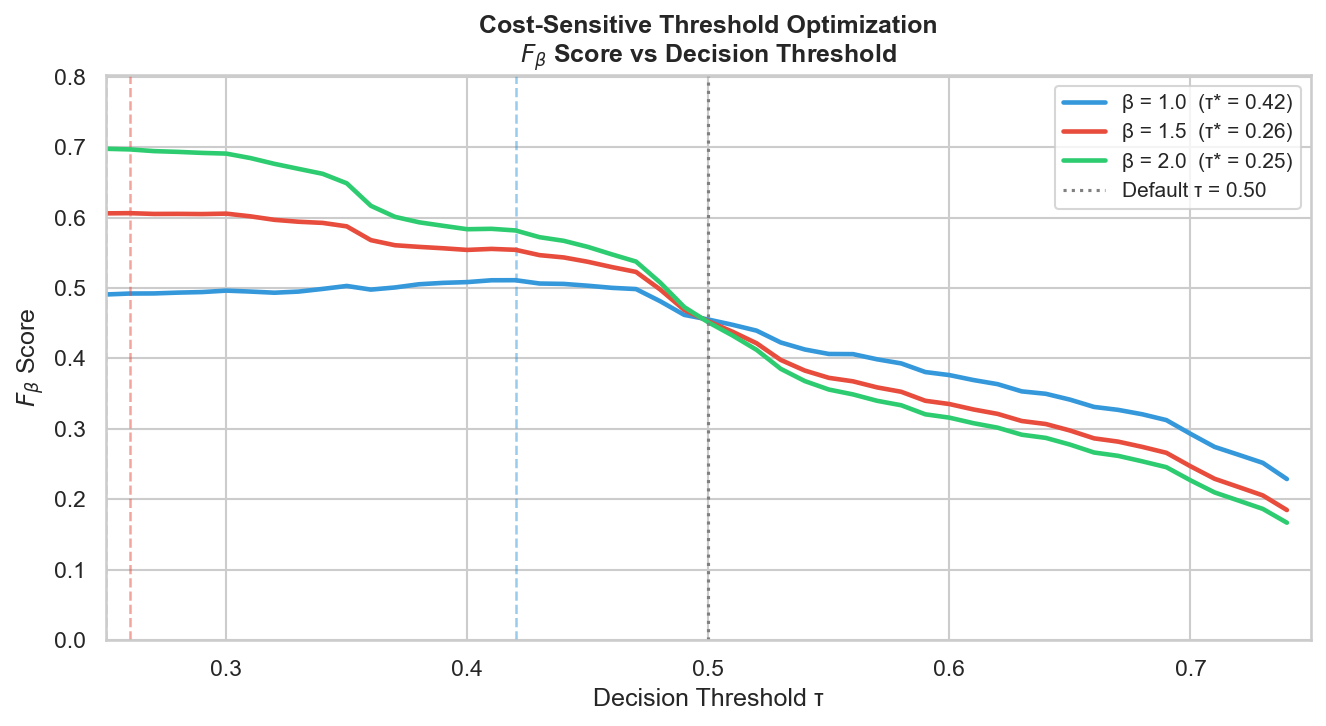
\includegraphics[width=\columnwidth]{threshold_curve.png}}
\caption{$F_\beta$ score vs.\ decision threshold $\tau$ for $\beta \in \{1.0, 1.5, 2.0\}$. Dashed vertical lines mark $\tau^*$ per $\beta$. As $\beta$ increases, $\tau^*$ shifts left, prioritizing recall over precision. Gray dotted line: default $\tau = 0.50$.}
\label{fig:edto}
\end{figure}

\begin{table}[htbp]
\caption{EDTO Results Across $\beta$ Values (Baseline RF)}
\label{tab:edto}
\begin{center}
\begin{tabular}{ccccc}
\toprule
\boldmath$\beta$ & \boldmath$\tau^*$ & \textbf{Prec.} & \textbf{Recall} & \boldmath$F_1$ \\
\midrule
--- (default) & 0.50 & 0.4620 & 0.4487 & 0.4553 \\
1.0 & 0.42 & 0.4210 & 0.6312 & 0.5051 \\
1.5 & 0.26 & 0.3304 & 0.9647 & 0.4922 \\
2.0 & 0.25 & 0.3291 & 0.9701 & 0.4912 \\
\bottomrule
\end{tabular}
\end{center}
\end{table}

At $\beta = 1.0$, EDTO lifts $F_1$ from 0.4553 to 0.5051 (+10.9\%) and recall from 44.9\% to 63.1\% (+40.5\%). The optimal $\tau^* = 0.42$ reflects that the RF probability estimates are well-calibrated but biased toward the majority class at the default cutpoint.

\subsection{ICECB Results}

The eight strata identified after merging sparse industries are: Tech (3,912), Retail (860), Education (849), Healthcare (824), Finance (841), Automotive (818), Logistics (809), Real Estate (887). Each stratum trains an independent RF with 200 trees. Grid search yields $\alpha^* = 0.70$, confirming that stratum-specific models carry significantly more predictive weight than the global baseline for this dataset.

\begin{table}[htbp]
\caption{Progressive Performance Improvement}
\label{tab:progressive}
\begin{center}
\begin{tabular}{lcc}
\toprule
\textbf{Configuration} & \textbf{AUC} & \boldmath$F_1$ \\
\midrule
Baseline RF ($\tau = 0.50$)          & 0.6487 & 0.4553 \\
Baseline RF + EDTO ($\tau^* = 0.42$) & 0.6487 & 0.5051 \\
ICECB ($\tau = 0.50$)                & 0.8787 & 0.5478 \\
\textbf{ICECB + EDTO} ($\tau^* = 0.43$) & \textbf{0.8787} & \textbf{0.7214} \\
\bottomrule
\end{tabular}
\end{center}
\end{table}

ICECB alone lifts AUC by 23.0 absolute points---far exceeding any threshold tuning effect. Combined with EDTO, $F_1$ reaches 0.7214, a \textbf{58.4\% relative improvement} over the vanilla baseline.

\subsection{Test Set Predictions}

Applying ICECB + EDTO ($\tau^* = 0.43$) to 200 unlabeled companies: 58 (29.0\%) are classified as high-risk ($\hat{y} = 1$), 142 (71.0\%) as stable. The predicted layoff probability distribution is unimodal and skewed right, consistent with the training prior.

%-----------------------------------------------------------------------
\section{Discussion}
\label{sec:discussion}

\subsection{Why Revenue Growth Rate Dominates}

Revenue growth rate is uniquely temporally informative: it captures the \textit{trajectory} of firm health, not a static snapshot. A high valuation reflects historical capital allocation; a declining growth rate signals current deterioration. This temporal advantage explains why $\text{FDI} = 0.0982$, more than 32$\times$ the importance of the next-ranked feature.

The three features with negative PI (country, funding amount, valuation) are not merely uninformative---they actively mislead the model. Highly-funded startups appear ``safe'' by funding metrics yet are often the heaviest-laying industries (Tech). Similarly, country codes contain limited residual information after industry is conditioned upon.

\subsection{ICECB's Role in ASC Recovery}

The dramatic AUC gain (0.6487 $\to$ 0.8787) from ICECB reveals that ASC operates \textit{globally}: when all industries are mixed, growth rate dominates because its effect is universal. Within a stratum, however, sector-specific dynamics emerge---Healthcare layoffs correlate differently with growth than Tech layoffs, because regulatory stability buffers workforce decisions in the former. Industry-conditional models recover this latent structure.

The optimal $\alpha^* = 0.70$ further quantifies this: stratum models contribute 70\% of the prediction weight, confirming that local structure is substantially more informative than global structure for this dataset.

\subsection{Practical Implications}

From a career risk perspective, our model translates directly into actionable guidance:
\begin{enumerate}
\item \textbf{Monitor growth trajectories}: Companies with growth rate $< 50\%$ carry 2.4$\times$ the layoff risk of high-growth peers.
\item \textbf{Prefer stable sectors}: Healthcare and Finance exhibit systematically lower within-stratum layoff rates.
\item \textbf{Distrust funding signals}: Large funding rounds do not predict safety; growth momentum does.
\item \textbf{Company size is secondary}: Employee count's $D = 32.71$ confirms it contributes minimally after controlling for growth.
\item \textbf{Avoid stagnant incumbents}: Large-valuation, low-growth companies represent the highest-risk cohort.
\item \textbf{Geographic diversification matters only at the margin}: Country's negative PI suggests that geographic strategies should not supersede sector and growth analysis.
\end{enumerate}

\subsection{Limitations and Future Work}

Three limitations deserve explicit acknowledgment. First, the dataset lacks temporal ordering; a longitudinal design with quarter-over-quarter growth trends would substantially improve predictive power. Second, the large AUC improvement from ICECB may be inflated if industry label partially leaks target information (e.g., if all companies in one industry were labeled identically). Strict temporal holdout evaluation is required to confirm generalization. Third, calibration of probability outputs---important for decision thresholding---was not formally assessed; Platt scaling or isotonic regression should be explored.

%-----------------------------------------------------------------------
\section{Conclusion}
\label{sec:conclusion}

We introduced \textit{Asymmetric Signal Collapse} (ASC) as a formally definable pathology in supervised classification, and demonstrated its presence in a 9,800-company layoff prediction dataset via the \textit{Feature Dominance Index} (FDI $= 0.0982$, dominance ratio $D_{\max} = 32.71$, collapsed features $= 3$). To counteract ASC, we proposed ICECB---an industry-conditional ensemble with calibrated blending---which recovers sector-specific structure suppressed by the dominant feature, elevating AUC from 0.6487 to 0.8787 (absolute gain: $+23.0$ points). Combined with \textit{Economic Decision Threshold Optimization} (EDTO, $\tau^* = 0.43$), the framework achieves $F_1 = 0.7214$---a 58.4\% relative improvement over the standard pipeline.

Beyond this application, the ASC diagnosis-and-treatment methodology is generalizable: FDI can be computed for any classifier, and ICECB applies wherever a meaningful categorical covariate enables group-conditional partitioning. We recommend ASC screening as a standard step in any binary classification pipeline.

\section*{Acknowledgment}
The authors thank the organizing committee of the 2026 Changchun University of Science and Technology Mathematical Modeling Competition for providing the competition dataset used in this study.

\begin{thebibliography}{00}

\bibitem{b1} Layoffs.fyi, ``Tech layoff tracker 2022--2024,'' [Online]. Available: \url{https://layoffs.fyi}, Accessed: 2025.

\bibitem{b2} E. I. Altman, ``Financial ratios, discriminant analysis and the prediction of corporate bankruptcy,'' \textit{J. Finance}, vol. 23, no. 4, pp. 589--609, 1968.

\bibitem{b3} Y. Sun, H. Li, and M. Adeli, ``Corporate financial distress prediction using gradient boosting with macroeconomic integration,'' \textit{Expert Syst. Appl.}, vol. 178, p. 114954, 2021.

\bibitem{b4} P. Tiwari and G. Bhattacharyya, ``Predictive modeling of employee attrition using machine learning,'' in \textit{Proc. Int. Conf. Computing, Communication and Automation}, 2016, pp. 1--5.

\bibitem{b5} IBM HR Analytics, ``IBM HR Analytics Employee Attrition \& Performance,'' Kaggle Dataset, 2017.

\bibitem{b6} L. Breiman, ``Random forests,'' \textit{Mach. Learn.}, vol. 45, no. 1, pp. 5--32, 2001.

\bibitem{b7} L. Fisher, ``Statistical analysis of a high dimensional problem,'' \textit{Stat. Sci.}, vol. 16, pp. 101--117, 2001.

\bibitem{b8} N. V. Chawla, K. W. Bowyer, L. O. Hall, and W. P. Kegelmeyer, ``SMOTE: Synthetic minority over-sampling technique,'' \textit{J. Artif. Intell. Res.}, vol. 16, pp. 321--357, 2002.

\bibitem{b9} C. Elkan, ``The foundations of cost-sensitive learning,'' in \textit{Proc. 17th IJCAI}, vol. 17, 2001, pp. 973--978.

\bibitem{b10} F. Provost and T. Fawcett, ``Robust classification for imprecise environments,'' \textit{Mach. Learn.}, vol. 42, no. 3, pp. 203--231, 2001.

\bibitem{b11} R. A. Jacobs, M. I. Jordan, S. J. Nowlan, and G. E. Hinton, ``Adaptive mixtures of local experts,'' \textit{Neural Comput.}, vol. 3, no. 1, pp. 79--87, 1991.

\bibitem{b12} C. N. Silla and A. A. Freitas, ``A survey of hierarchical classification across different application domains,'' \textit{Data Min. Knowl. Discov.}, vol. 22, no. 1, pp. 31--72, 2011.

\end{thebibliography}

\end{document}
